\section{Preliminaries}
\label{sec:prelim}

In this section, we define the terminologies used in the paper and give a formal definition of the problem under consideration. In addition, we analyze the complexity of the problem and its hardness.

\subsection{Problem Definition}
\label{subsec:problemdef}

We start by defining some terminologies in order to formally define the task assignment problem in spatial crowdsourcing.

\begin{definition} [Spatial Task]
A spatial task t shown as $\left\langle l, [r, d] \right\rangle$ is a task to be performed at location l with geographical coordinates, i.e., latitude and longitude. The task becomes available at r (release time) and expires at d (deadline).
\end{definition}

It should be pointed out that in a spatial crowdsourcing environment, a spatial task \emph{t} can be executed only if a worker is at location \emph{t.l}. For example, if the query is to report the traffic situation at a specific location, someone has to actually be present at the location to be able to report the traffic. Hereafter, whenever we use \emph{task} we are referring to a spatial task. Now, we formally define a worker.

\begin{definition} [Worker]
A worker w shown as $\left\langle l, T, max, [s, e] \right\rangle$ is any entity, e.g., a person, willing to perform spatial tasks. We show the current location of the worker by w.l. Each worker has a list of tasks assigned to it, w.T, and a maximum number of tasks it is willing to perform, w.max. Also w.s and w.e show the availability of the worker such that the worker is available during the time interval $\left( w.s, w.e \right]$.
\end{definition}

Throughout the paper we assume every worker moves one unit of length per unit of time. Therefore, we can assume that $distance \left( \left\langle a,b \right\rangle \right)$ is also the \emph{time} required to move from point $a$ to point $b$.

\begin{definition} [Schedule]
We call an ordered list of tasks a schedule. We show s as $\left\langle t_1, ..., t_n \right\rangle$ where n is the number of tasks in s. If we show the $i^{th}$ task in s with $s_i$, we say worker w is able to perform schedule s if and only if:
\begin{equation*}
\forall i, 1\leq i \leq n \ \ \ \ \sum_{j=1}^i distance(s_{j-1}, s_j) \leq s_i.d
\end{equation*}
where $s_0$ represents the current location of $w$.
\end{definition}

At each point in time, each worker keeps track of a schedule and completes the tasks based on their order in its schedule.

\begin{definition} [Matching]
Assuming we have a set of workers W and a set of tasks T, we call $M \subset W \times T$ a matching if for each $t \in T$ there is at most one $w \in W$ such that $\left( w, t \right) \in M$. We call $\left( w, t \right) \in M$ a \emph{match} and say t has been matched to w. For each matching M, we define the value (benefit) of M as:
\begin{equation*}
Value(M) = \vert M \vert
\end{equation*}
\end{definition}

\noindent A matching $M$ is valid if and only if, for every worker $w$, there exists a schedule $s$, such that $(w, t_i) \in M \implies t_i \in s$. 

Now we can formally define the Task Assignment in Spatial Crowdsourcing (TASC) as follows:

\begin{definition}[Task Assignment in SC]
Given a set of workers $W$, a set of spatial tasks $T$ and a cost function $d: \left( W \cup T \right) \times T \rightarrow \mathbb{R}$ where $d \left( \left\langle a,b \right\rangle \right)$ is the distance between $a$ and $b$, the goal of the TASC$\left\langle W, T, d \right\rangle$ problem is to find a valid matching $M$ with maximum value.
\end{definition}

It is important to note that with task assignment in SC, the goal is to find a \textit{valid matching}. This means that in addition to finding a \textit{matching} between tasks and workers, the SC-Server has to also find a \textit{schedule} for each worker to perform the tasks. Throughout this paper we use the terms \textit{matching phase} and \textit{scheduling phase} to refer to the two different aspects of task assignment in SC. \cref{tab:notation} lists the notations we frequently use in this paper.\\

\begin{table}
\begin{center}
\begin{tabular}{| c | l |} \hline
Notation	&	Description \\ \hline
$t.l$		&	location of task $t$ \\ \hline
$t.r$		&	release time of task $t$ \\ \hline
$t.d$		& 	deadline of task $t$ \\ \hline
$w.l$		&	location of worker $w$ \\ \hline
$w.s$		&	the time worker $w$ becomes available \\ \hline
$w.e$		&	the time worker $w$ becomes unavailable \\ \hline
$w.T$		&	list of tasks assigned to worker $w$ \\ \hline
$w.max$		&	maximum number of tasks worker $w$ \\
			&	performs \\ \hline
\end{tabular}
\caption{List of notations}
\label{tab:notation}
\end{center}
\end{table}

\subsection{Complexity Analysis}

\begin{theorem}
\label{th:comp_ratio}
There does not exist a deterministic online algorithm for the TASC problem that is \textit{c-competitive} ($c > 0$). 
\end{theorem}

\begin{proof}
Suppose there exists an algorithm $\mathcal{A}$ that is \textit{c-competitive}. We assume there exist a Clairvoyant which knows every decision $\mathcal{A}$ makes. For simplicity, we assume there is only one worker at point $(0, 0)$. The input starts with $r_1$ with a pick-up location at $(w, 0)$ and $r_2$ with pick-up location at $(-w, 0)$ (we assume all requests have a maximum wait time of $w$). The algorithm can make three choices for the driver. (1) move toward $r_1$, (2) move towards $r_2$ and (3) stay still. If choice 1 is selected, the Clairvoyant can generate the input such that at time $t = 1$, $n$ more request are submitted with pick-up location at $(-w-1, 0)$ and drop-off locations similar to $r_2$. Similar arguments can be made if choice 2 or 3 are selected by the algorithm. A globally optimal solution can complete $n+1$ requests while $\mathcal{A}$ can at most complete one request. By adding more drivers far away in a similar situation, the Clairvoyant can make $\mathcal{A}$'s solution unboundedly worse than the optimal solution. Therefore, we contradicted the assumption that $\mathcal{A}$ is \textit{c-competitive}.
\end{proof}

\begin{figure}[h]
    \centering
    \subfigure[$t = 0$]{
        \label{fig:prooft0}
        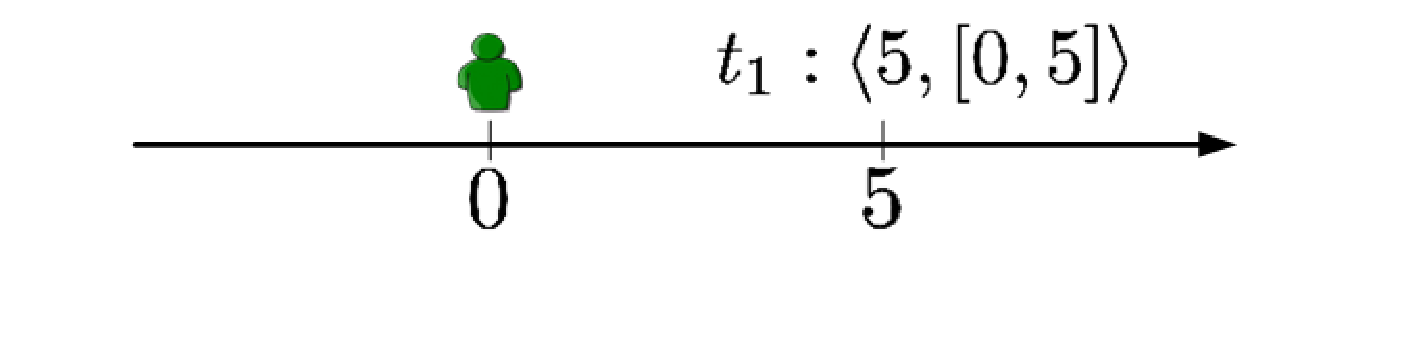
\includegraphics[width = 0.9\columnwidth]{figures/proof0}
    }
    \subfigure[$t = 2$, case $1$]{
        \label{fig:prooft21}
        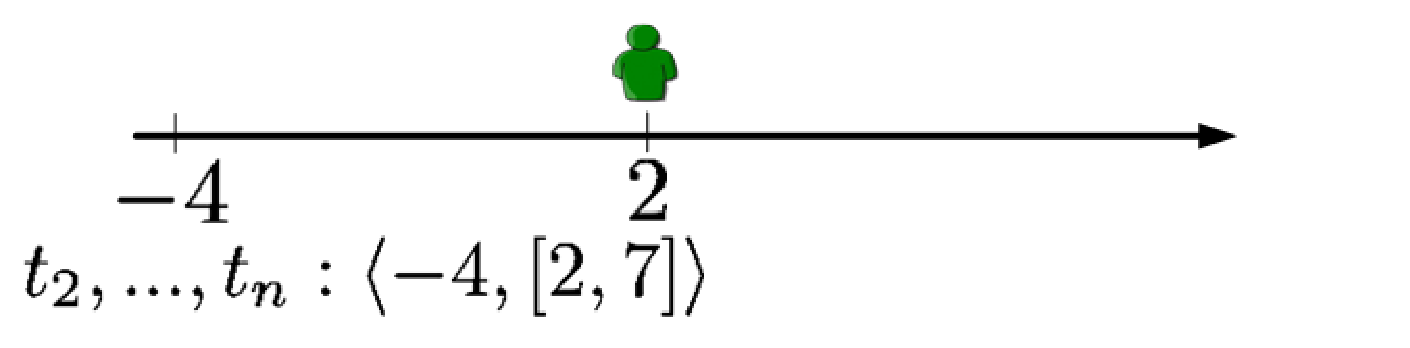
\includegraphics[width = 0.9\columnwidth]{figures/proof21}
    }
    \subfigure[$t = 2$, case $2$]{
        \label{fig:prooft22}
        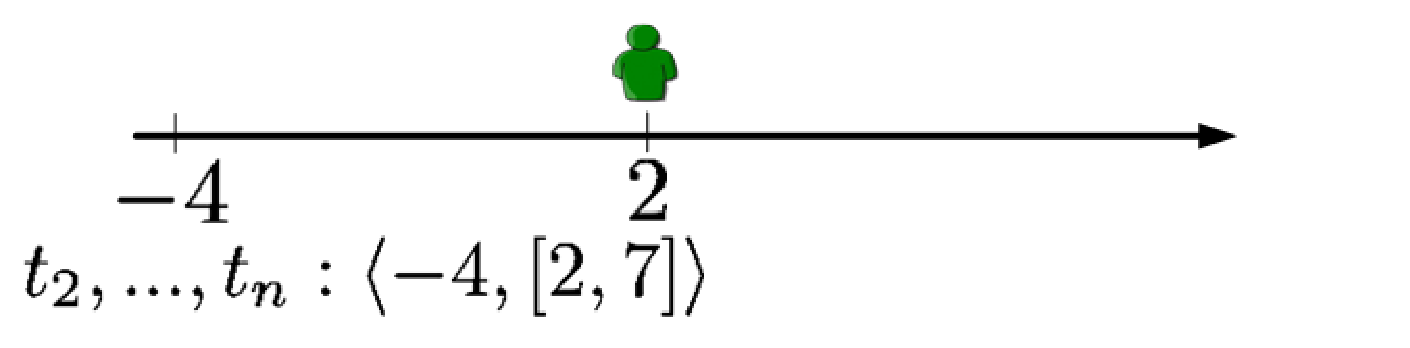
\includegraphics[width = 0.9\columnwidth]{figures/proof22}
    }
    \vspace{-0.15in}
    \caption{Adversary Generated Input}
    \label{fig:quality}
\end{figure}
%The equivalent decision problem for TASC is to decide if there exists a matching $M$ with value $K$ and is denoted as TASC$\left\langle W, T, d, K \right\rangle$. In this section we use a slightly modified version of the well known Hamiltonian Path Problem. We call it the Minimum Length Hamiltonian Path Problem (Min-Ham-Path) and define it as follows:

%\begin{definition}[Min-Ham-Path]
%Given a directed graph $G(V,E)$ where each edge $e \in E$ is assigned a length $l: E \rightarrow \mathbb{R}$, a source node $s$ and a length $L \in \mathbb{R}$, the Min-Ham-Path problem $\left\langle G, l, s, L \right\rangle$ is to decide whether there exists a path in $G$ that starts from $s$, visits every other node exactly once and has a length of at most $L$.
%\end{definition}

%\begin{theorem}
%\label{th:MinHam}
%The Min-Ham-Path problem is NP-Hard.
%\end{theorem}

%\begin{proof}
%Proof is shown in \cref{app:MinHamProof}.
%In order to prove the NP-Hardness of Min-Ham-Path we show Ham-Path $\leq_p$ Min-Ham-Path. The Hamiltonian Path problem asks the following question: Given a directed graph $G(V,E)$ does there exist a path that goes through every node exactly once?

%Given an instance of the Ham-Path problem $\left\langle G \right\rangle$ we modify graph $G(V,E)$ and generate a new graph $G'(V', E')$ where $V' = V \cup \left\{ o \right\}$ and $E' = E \cup \left\{ \left\langle o, v \right\rangle : v \in V \right\}$. Also, for every $e \in E'$ we Assume $l(e) = 1$.

%Now we show that Ham-Path$\left\langle G \right\rangle$ is true if and only if Min-Ham-Path$\left\langle G', l, o, n \right\rangle$ is true where $n$ is the number of vertices in $G$. If Min-Ham-Path returns a path of length $n$, we can remove the first edge from the path which results in a Hamiltonian Path for the Ham-Path$\left\langle G \right\rangle$ problem. On the other hand every Hamiltonian Path on graph $G$ has length $n-1$. By adding vertex $o$ and connecting it to the starting vertex, we end up with a Hamiltonian Path of length $n$ on $G'$.
%\end{proof}

%\begin{theorem}
%\label{th:TASC}
%The TASC problem is NP-Complete.
%\end{theorem}

%\begin{proof}
%Proof is shown in \cref{app:TASCProof}
%We start the proof by showing that the decision problem of TASC is \textit{verifiable} in polynomial time. Given a matching $M$, we can check that no task is assigned to more than one worker in polynomial time. Furthermore, based on the definition of a valid match, checking the validity of a matching $M$ can be done in polynomial time as well. Finally, we can find the value of $M$ by adding the value of every task in $M$.

%We show TASC is NP-Hard by proving the reduction Min-Ham-Path $\leq_p$ TASC. Given an instance of the Min-Ham-Path problem $\left\langle G(V,E), l, o, K \right\rangle$ we reduce it to an instance of the TASC$\left\langle W, T, l', n-1 \right\rangle$ problem such that $W = \left\{ o \right\}$, $T = V \setminus \left\{ o \right\}$. For every task $t$ we set $t.v = 1$, $t.r = 0$ and $t.d = K$. Also for every $e \in E, l'(e) = l(e)$. In addition for every $e' \in \left( W \times T \right) \cup \left( T \times T \right) $ where $e' \not\in E$ we set $l'(e') = \infty$.

%Finally we show the result of Min-Ham-Path$\left\langle G, l, o, K \right\rangle$ is true if TASC$\left\langle W, T, l', n-1 \right\rangle$ is true where $n$ is the number of vertices in $G$. Considering that $\left\vert T \right\vert = n - 1$ and $t.v = 1$ for every $t \in T$, if there exists a matching with size $n - 1$ it means every task has been assigned to the single worker. Also, since the deadline of every task is $K$ the worker visits every task no later than $K$. Therefore, the path that the worker traverses starts at $o$ and goes through every other vertex $v \in V \setminus \left\{ o \right\}$, where the length of the path is no more than $K$.
%\end{proof}